\documentclass[11pt]{article}

% Packages
\usepackage{amsmath,amssymb}
\usepackage{graphicx}
\usepackage{hyperref}
\usepackage{caption}
\usepackage{subcaption}
\usepackage{booktabs}
\usepackage{multirow}
\usepackage{array}
\usepackage[top=1in, bottom=1in, left=1in, right=1in]{geometry}
\usepackage{xcolor}
\usepackage{float}
\usepackage{enumitem}
\usepackage{mathtools}
\usepackage{microtype}

% Title and author information
\title{Trends in Frontier AI Model Count: A Forecast to 2028}
\date{\today}

\begin{document}

\maketitle

\begin{abstract}
Governments are starting to impose requirements on AI models based on how much compute was used to train them. For example, the EU AI Act imposes requirements on providers of general-purpose AI with systemic risk, which includes systems trained using greater than $10^{25}$ floating point operations. In the United States' AI Diffusion Framework, a training compute threshold of $10^{26}$ is used to identify ``controlled models'' which face a number of requirements. We explore how many models such training compute thresholds will capture over time. We estimate that by the end of 2028, there will be between 81-287 foundation models exceeding the $10^{25}$ FLOP threshold put forward in the EU AI Act (90\% CI), and 37-134 models exceeding the $10^{26}$ FLOP threshold that defines controlled models in the AI Diffusion Framework (90\% CI). We also find that the number of models exceeding these absolute compute thresholds each year will increase superlinearly -- that is, each successive year will see more new models captured within the threshold than the year before. Thresholds that are defined with respect to the largest training run to date (for example, such that all models within one order of magnitude of the largest training run to date are captured by the threshold) see a more stable trend, with 5-350 (90\% CI) being captured by this definition each year.
\end{abstract}

\section{Introduction}

Recent years in machine learning have seen the rise of foundation models -- AI systems that exhibit powerful and general-purpose capabilities. Governments across the world have started to impose requirements on the development and deployment of the most capable such systems, such as the GPT o-series\footnote{\href{https://openai.com/o1/}{Introducing OpenAI o1}}. In December 2023 the European Union adopted the EU AI Act, the world's first comprehensive legislation designed to govern the development and use of AI systems. Among other things, the Act imposes requirements on providers of general-purpose AI with systemic risk (GPAISR), as of August 2025, which includes systems trained using greater than $10^{25}$ floating point operations (FLOP)\footnote{In this paper we often use the notation $10^X$ to refer to absolute compute thresholds. However the notation 1eX also appears at times which is interchangeable with the first notation. For 1e24 FLOP = $10^{24}$ FLOP, 5.3e25 FLOP = $5.3 \times 10^{25}$ FLOP, etc.}. The European Union is not the only jurisdiction to impose requirements based on \href{https://arxiv.org/abs/2405.10799}{training compute thresholds}; in one of its final acts the Biden administration issued the Artificial Intelligence Diffusion Framework\footnote{\href{https://www.federalregister.gov/documents/2025/01/15/2025-00636/framework-for-artificial-intelligence-diffusion}{Federal Register :: Framework for Artificial Intelligence Diffusion}}, which as one of its key directives introduced a host of requirements on models above $10^{26}$ FLOP (named ``controlled models'' in the framework) with the aim of maintaining leadership in AI technology amongst the US and its allies.

However, it is well established that the training compute used for frontier models has been growing extraordinarily quickly,\footnote{\href{https://epochai.org/blog/training-compute-of-frontier-ai-models-grows-by-4-5x-per-year}{Training Compute of Frontier AI Models Grows by 4-5x per Year}} with mean model size growing by about 4-5x per year over the past decade. This has important implications for compute-based regulations such as those included in the EU AI Act and the Diffusion Framework. In April 2025, \underline{\href{https://epochai.org/data/notable-ai-models}{estimates suggest}} that there are 2 publicly available models trained using more than $10^{26}$ FLOP and over 20 publicly available models trained using more than $10^{25}$ FLOP. However, if current trends continue, these numbers may quickly grow. Governments need to take into account this growth in their AI governance efforts. By underestimating the number of models covered by their thresholds, they may fail to build sufficient regulatory capacity to implement their regulations or may impose regulatory burdens on an excessive number of actors.

With this in mind, in the following paper we estimate the number of released models that will exceed various compute thresholds over the coming years. Extrapolating from current trends we conclude that by the end of 2028 there could be between 81-287 \hyperref[results]{models exceeding the} $10^{25}$ \hyperref[results]{FLOP threshold (90\% confidence interval), and 37-134 models exceeding the} $10^{26}$ \hyperref[results]{FLOP threshold (90\% confidence interval)}. We also study ``frontier-connected thresholds'' -- thresholds that are defined relative to the largest training run at any one point in time rather than based on the absolute amount of training compute used -- and find that in the coming years there will be between 5-30 models within 1 OOM of the largest training run that has taken place (90\% CI). However our analysis has limitations resulting from \hyperref[notable-models-selection-effect]{selection effects in the database that we extrapolate trends from}, as well as uncertainty in key parameters that have influence the projections.

Importantly, our estimates do not straightforwardly translate into the number of models in scope of the EU AI Act or AI Diffusion Framework. Our numbers may provide an overestimate in that neither the EU nor the US would apply to models trained and only made available in other jurisdictions (e.g., China). Additionally, the AI Act only applies to general purpose AI - it is unclear whether image and video generation models (such as OpenAI's SORA or Google DeepMind's Imagen\footnote{\href{https://openai.com/sora/}{https://openai.com/sora/} \href{https://deepmind.google/technologies/imagen-3/}{Imagen - Google DeepMind}}) would count as GPAI. The Act may also not apply to models that were placed on the market before the relevant obligations come into force in August 2025. Further, both rules could affect the market for AI development, making it less attractive for companies to release in-scope models. If these effects occur, our analysis may end up over counting the models captured by these thresholds. At the same time, our estimates may underestimate the number of models subject to the compute-based threshold requirements. This is because the regulation could apply not only to original GPAISR developers but also to companies that modify the models\footnote{\href{https://arxiv.org/abs/2503.11922}{[2503.11922] On Regulating Downstream AI Developers}}, for example by adding software infrastructure around the model to make an AI agent\footnote{Chan, Alan, et al. ``Infrastructure for AI Agents.'' \href{https://arxiv.org/abs/2501.10114}{arXiv preprint arXiv:2501.10114 (2025).}}. Since our analysis does not account for such adaptations, the actual number of affected models could be higher than our estimates suggest. Finally it should be noted that the EU AI Office has the ability to update the threshold in both directions - as does the US Bureau of Industry and Security in the U.S. as it relates to the AI Diffusion Framework - which would have to be taken into consideration when interpreting the predictions in future years.

\section{Methodology}

Our aim is to forecast the number of models that will be released above different training compute thresholds over the next four years. To do this, we model scenarios for how the distribution of model size over training compute evolves. Once these distributions are established, we can simply count the models that exceed each specific compute threshold.

\subsection{Data}

We use Epoch AI's \underline{\href{https://epoch.ai/data/notable-ai-models-documentation#:~:text=Changelog\%20Downloads\%20Acknowledgements-,Overview,and\%20future\%20of\%20artificial\%20intelligence.}{Notable Models dataset}} as the main dataset for our analysis. To our knowledge, this is the most comprehensive publicly available dataset of machine learning models available with over 450 entries of models and their estimated training compute. However, it is important to note that ML models must satisfy one of the following four criteria (the \textit{notability criteria}\footnote{\href{https://epoch.ai/data/notable-ai-models-documentation#inclusion}{Notable AI Models Documentation | Epoch AI}}) to be included in the database:

\begin{itemize}
\item highly cited (over 1000 citations);
\item large training cost (over \$1,000,000, measured in 2023 USD);
\item significant use (over one million monthly active users);
\item state of the art performance (typically on a recognised ML benchmark);
\item indisputable historical significance.
\end{itemize}

This makes the notable models dataset a strict subset of all \textit{machine learning models,} and the selection effect applied by the notability criteria should be accounted for when interpreting the results in this paper. In short, this selection effect biases our median estimates towards being a lower bound estimate, especially for models that are multiple orders of magnitude of training compute below frontier models\footnote{This is because models multiple orders of magnitude away from the frontier are less likely to be captured by the notable model criteria relative to models close to the frontier.}. For these models that are significantly smaller than the frontier models, it is also difficult to quantitatively estimate the extent to which the estimates derived from the notable models database will be lower than the actual value. However, anchoring on the full 90\% prediction intervals presented in the \underline{\hyperref[results]{Results}} section provides \textit{some} insurance against the effects of this selection effect (i.e: in some cases the 95th percentile projection is likely to be closer to the actual number of models exceeding the compute threshold). The effects of the Notable Model database selection effects, and how this can be accounted for within our model are discussed in further detail in the \underline{\hyperref[notable-models-selection-effect]{limitations}} section.

Whilst the Notable Models database contains $\sim$450 entries with associated training compute values from 2010-2024, we fit our model based on the data from 2017-2023 (with 296 datapoints) to capture recent trends in the field. We do not use 2024 data to fit the model as the data is more likely to be incomplete - this is because the models tracked in the database lag behind models released by a handful of months. Visualisations of the model distribution in the dataset provide evidence in support of this, and are shown in \underline{\hyperref[appendix-a-historical-distribution-of-notable-models-and-fit-data-choice]{Appendix A}}.

\subsection{Allocating total compute spending across different model scales}

We forecast the distribution of models over training compute by projecting the total amount of compute that will be spent training AI models in the coming years, and then modelling how this compute stock is distributed over models of different size. We choose this approach as we expect the \textit{total} training compute spending to be a strong and relatively simple-to-forecast constraint on model distributions (over training compute). The allocation of compute to models of different sizes also exhibits a linear trend that is simple to extrapolate (discussed below).

Note that there are alternate ways to estimate the future distribution of models over training compute; for example, one could fit a parametric distribution (e.g: a normal distribution) to historical data, extrapolate this into future years and then sample from this distribution. However we do not use this method for the following reasons: Firstly, it is unclear which parametric distributions, if any, are a good \underline{\hyperref[appendix-a-historical-distribution-of-notable-models-and-fit-data-choice]{fit to historical distributions}} of training compute. Secondly, our approach has a more explicit focus on determining model distributions from total training compute spending - which, as mentioned above, we expect to be a strong and simple-to-forecast constraint over the next few years.

Using our approach, we project future model distributions over training compute by:

\begin{enumerate}
\item Exponentially projecting the total compute that will be used for AI workloads (both training and inference) with a median annual growth rate of roughly 4.1x.

\item Allocating this compute with a split of 40\% of compute towards model training and 60\% of compute towards other uses (inference and research experiments) in 2025 and 2026, and a 30-70 allocation in 2027 and 2028.

\item Allocating the training compute across models of different scales - i.e: models within 1 OOM of the frontier model, models within 1 and 2 OOMs of the frontier model, models within 2 and 3 OOMs of the frontier model etc. - by fitting to data from 2017-2023 and assuming these allocation trends hold over the coming years.
\end{enumerate}

We will now discuss each of these in turn in greater detail.

We first begin by projecting the total amount of compute that will be used for AI workloads (training and inference) in the coming years. We use two sources for this.

Firstly, we can look at historical growth rates of training compute from the Notable Models database. Doing so for the years that we fit the model (2017-2023), we find a rapid growth rate of 6.3x annually for the total training compute used to train AI models. \textit{Assuming that the historical allocation between model training and inference has stayed roughly constant (at \underline{\hyperref[allocating-compute-between-training-inference-and-other-workloads]{40-60}}),} we can generalise this to a 6.3x growth in compute used for AI workloads.

On the other hand, Dean et al.\footnote{\href{https://ai-2027.com/research/compute-forecast}{Compute Forecast --- AI 2027}} model the growth in compute for AI workloads as increasing at a rate of 3.4x per year. This is the compound growth rate resulting from a 2.25x increase per year of the compute stock that \textit{can} be used for AI workloads, and a 1.5x increase per year of the \textit{share} of this stock that actually is allocated to AI training and inference\footnote{One can think of these two quantities as AI compute \textit{capacity} and AI compute \textit{usage.}}. The 2.25x growth rate in global AI-relevant compute stocks results from a 1.35x growth rate in the physical stock of AI chips and 1.65x in chip efficiency\footnote{\href{https://ai-2027.com/research/compute-forecast}{Compute Forecast --- AI 2027}}. The 1.5x growth in share results from aggressive build outs of data centres by leading AI developers, financed by revenues on the order of tens of billions of dollars resulting from highly performant AI models and agents.

Given the discrepancy between these two estimates we integrate both into our median growth rate forecast. We put more weight on the 3.4x per year increase in compute for AI workloads given the detailed analysis that leads to this figure, however we do not fully discount the rapid growth rate that has been historically observed. Specifically we give the 3.4x figure three times as much weight as the historically observed figure, but this weighting is subjective and predictions for alternative growth rates are shown in \underline{\hyperref[appendix-g-results-for-varying-growth-rate-weightings]{Appendix G}}. Applying this weighting between the two growth rates leads to a median growth rate of the AI workload stock (i.e: the stock of compute used for AI training and inference) of 4.1x per year. To account for uncertainty in the actual annual growth rate of compute for AI workloads, we add noise to the median growth rate, drawn from a normal distribution with mean of 0 and standard deviation of 0.5.

Next, we model (a) how the AI compute stock is allocated between training and inference and (b) how the total training compute is allocated across models of different sizes. In this analysis we project two scenarios for part (a) -- one in which the allocation remains the same as previous years, and another in which we see an increasing fraction of compute allocated to model inference; this is discussed in further detail \underline{\hyperref[allocating-compute-between-training-inference-and-other-workloads]{here}}. To answer (b), we look at how training compute has been allocated to models of different sizes in recent years, and assume that these allocation trends hold in the coming years. This approach means that we do not have to explicitly commit to fixed parametric distributions.

\underline{\hyperref[figure-2a-compute-allocation-across-model-sizes-for-years-2020-2023-x-axis-unnormalised.]{Figure 2A}} below shows how training compute spending in the years 2020-2023 has been allocated to models of different sizes (data for 2017-2019 are shown in \underline{\hyperref[appendix-b-compute-allocations-for-2017-2019]{Appendix B}}). The x-axis represents the size of individual models. The y-axis shows the fraction of training compute spent training models of size m or less. Differences in model sizes and their compute share can span orders of magnitude so both axes are log-scaled.

\begin{figure}[h]
\centering

\includegraphics[width=0.8\textwidth]{media/image4.png}
\caption*{\textbf{Figure 2A}: Compute allocation across model sizes for years 2020-2023, x-axis unnormalised.}
\label{figure-2a-compute-allocation-across-model-sizes-for-years-2020-2023-x-axis-unnormalised.}
\end{figure}

To get a concrete sense of what the plot shows, here are some conclusions that can be made by reading off the graph:

\begin{itemize}
\item In 2021, models of size $10^{22}$ FLOP or less contributed to approximately 1\% of total compute spending.
\item In 2021, models of size $10^{21}$ FLOP or less contributed approximately 0.1\% of total compute spending
\item In 2022, models of size $10^{21}$ FLOP or less contributed approximately 0.01\% of total compute spending
\item In 2023, models of size $10^{23}$ FLOP or less contributed just less than 10\% total training compute spending.
\end{itemize}

\underline{\hyperref[figure-2a-compute-allocation-across-model-sizes-for-years-2020-2023-x-axis-unnormalised.]{Figure 2A}} also marks the largest model trained each year with the red vertical line. By definition, the largest model and all those smaller than it account for 100\% of compute spending in a given year; this is shown in \underline{\hyperref[figure-2a-compute-allocation-across-model-sizes-for-years-2020-2023-x-axis-unnormalised.]{Figure 2A}} by the fact that this line intersects with the line representing total compute spending.

The relationship between model size m and total compute spent training models of size m or less is consistently linear across 2020-2023 (and \underline{\hyperref[appendix-b-compute-allocations-for-2017-2019]{2017-2019}}), suggesting a stable trend that we can extrapolate. The size of individual models grows each year, so to extrapolate this trend we normalise the x-axis by the largest model trained in each year (shown in \underline{\hyperref[figure-2b-compute-allocation-amongst-model-sizes-for-years-2020-2023-x-axis-normalised-by-largest-model-trained-that-year.-linear-fit-shown.]{Figure 2B}}). Table 1 shows the compute allocations for different model sizes for 2023 that are derived from these plots.

\begin{figure}[h]
\centering
\includegraphics[width=0.8\textwidth]{media/image5.png}
\caption*{\textbf{Figure 2B}: Compute allocation amongst model sizes for years 2020-2023, x-axis normalised by largest model trained that year. Linear fit shown.}
\label{figure-2b-compute-allocation-amongst-model-sizes-for-years-2020-2023-x-axis-normalised-by-largest-model-trained-that-year.-linear-fit-shown.}
\end{figure}

\begin{table}[h]
\centering
\caption*{\textbf{Table 1}: 2023 allocations -- Largest model: Gemini Ultra @ 5x10$^{25}$ FLOP, total compute = 1.35x10$^{26}$ FLOP. We use OOM to refer to an order of magnitude of training compute. Allocations may not sum exactly to 1 due to rounding errors.}
\label{table-1-2023-allocations-largest-model-gemini-ultra-5x1025-flop-total-compute-1.35x1026-flop.-we-use-oom-to-refer-to-an-order-of-magnitude-of-training-compute.-allocations-may-not-sum-exactly-to-1-due-to-rounding-errors.}
\begin{tabular}{|p{2cm}|p{2cm}|p{2cm}|p{2cm}|p{2cm}|p{2cm}|}
\hline
\multicolumn{6}{|c|}{\textbf{Compute allocation in 2023}} \\
\hline
Model size relative to Gemini Ultra (5x10$^{25}$ FLOP) & All models within 5 OOM - 4 OOM & All models within 4 OOM - 3 OOM & All models within 3 OOM - 2 OOM & All models within 2 OOM - 1 OOM & All models within 1 OOM \\
\hline
Model size (absolute) & 5$\times$10$^{20}$ - 5$\times$10$^{21}$ & 5$\times$10$^{21}$ - 5$\times$10$^{22}$ & 5$\times$10$^{22}$ - 5$\times$10$^{23}$ & 5$\times$10$^{23}$-5$\times$10$^{24}$ & 5$\times$10$^{24}$ - 5$\times$10$^{25}$ \\
\hline
Fractional allocation of total compute (2 s.f.) & 0.00011\% & 0.0010\% & 0.010\% & 8.6\% & 90\% \\
\hline
Compute allocation (FLOP) & 1.51$\times$10$^{22}$ & 1.43$\times$10$^{23}$ & 1.36$\times$10$^{24}$ & 1.16$\times$10$^{25}$ & 1.22$\times$10$^{26}$ \\
\hline
\end{tabular}
\end{table}

Before moving on, It is worth briefly considering the constraints and physical interpretations of the parameters of the linear fits - namely, the gradient (k) and the intercept (b).

First, note that the linear fits must pass through (1,1) on the normalised plots (Figure 2B) - this is because, by definition, the largest model and all models smaller than it (i.e: all models released in a given year) account for 100\% of compute used. This means that the intercept of the linear fits - b - must be 0 (see \underline{\hyperref[appendix-c-constraints-and-interpretation-of-the-linear-fits]{Appendix C}} for details). Regarding k, \underline{\hyperref[appendix-c-constraints-and-interpretation-of-the-linear-fits]{Appendix C}} shows that models that are 10x the size of a smaller counterpart are allocated roughly 10$^k$ times as much compute. Historical values for k are seemingly equally distributed across the range [0.9, 1.1] (\underline{\hyperref[appendix-d-historical-values-of-allocation-gradients]{Appendix D}}), therefore our model samples k uniformly from the range [0.9,1.1]. The edge case of k=0.9 corresponds to models that are 10x as large as a counterpart being allocated 10$^{0.9}$ = $\sim$8.0 times as much compute, whereas the factor for the k=1 case is 10$^{1.1}$ = 12.6 times as much compute.

Finally, observing \underline{\hyperref[table-1-2023-allocations-largest-model-gemini-ultra-5x1025-flop-total-compute-1.35x1026-flop.-we-use-oom-to-refer-to-an-order-of-magnitude-of-training-compute.-allocations-may-not-sum-exactly-to-1-due-to-rounding-errors.]{Table 1}} closely shows that our model requires an assumption to be made about the size of the largest model released in a given year in relation to the total training compute spending that year. This parameter is referred to as the largest model share (or LMS parameter) in the rest of this analysis. Observing this parameter from the years we fit the model to (\underline{\hyperref[f.1-historical-lms]{Appendix F.1}}) leads us to sampling the LMS uniformly from the range [0.05, 0.5] except for the year 2024 where we set the largest model to the size of GPT-4o (3.8x10$^{25}$ FLOP, released May 2024) following the data in the Notable models database. Concretely, this means that in the years 2025-2028 we assume that the largest training run uses at most 50\% of the training compute stock that year, and at least 5\%. A 50\% share of the total training compute used may initially appear large, but similar scenarios are not historically unprecedented, with the Notable Models database documenting that GPT-3 175B davinci (3.14$\times$10$^{23}$ FLOP) accounted for $\sim$46\% of the 6.75$\times$10$^{23}$ FLOP of training compute that year.

Our modelling choices for the LMS parameter for 2024 are discussed further in \underline{\hyperref[appendix-e-2024-predictions-under-uniform-sampling-of-lms]{Appendix E}}. The LMS parameter is an important input to our model and its influence on the model's predictions are discussed further in \underline{\hyperref[f.2-influence-of-lms-on-projections]{Appendix F.2}}.

Finally, to generate model distributions to extend the historical data we randomly sample models from each bin until the total training compute allocated to that bin is met or exceeded.

\subsection{Allocating compute between training, inference, and other workloads}
\label{allocating-compute-between-training-inference-and-other-workloads}

Given estimates of the total compute stock, the next key stage involves allocating this stock between training, inference and other workloads. First a note on the different usages for compute. AI developers can use compute for model training (both pre- and post-training), as well as serving models to customers ('external' deployment/inference), using models in-house for research automation and monitoring ('internal' deployment/inference), compute for research experiments, generating synthetic data, and more. For this analysis, it is sufficient to categorise compute usage into 'training' and 'inference' following existing analyses\footnote{\href{https://epoch.ai/gate}{GATE Model Playground | Epoch AI}}, though it's important to note that 'inference' here encompasses model inference and other related uses (such as synthetic data generation).

Dean et al.'s compute forecast\footnote{\href{https://ai-2027.com/research/compute-forecast}{Compute Forecast --- AI 2027}} estimates that in 2024 approximately 40\% of compute was used for training (including both pre- and post-training), with the remaining share going to model inference and other uses. This is used as the starting point for the model. Dean et al. then estimate the share of compute allocated to training in the following years, estimating that in 2025 and 2026 40\% of compute will be used for model training, 30\% at the start of 2027 and 20\% by the end of 2027. These allocations are mapped to the predictions years for this forecast (2025-2028) in the first column of \underline{\hyperref[table-2---compute-allocations-for-training-models-for-2025-2028.]{Table 2}}\footnote{Concretely, we take the start of 2027 allocation (30\%) as the allocation for all of 2027, and the end of 2027 allocation (20\%) as the 2028 allocation.}. The 20-80 allocation of compute between training and other uses at the end of 2027 represents an aggressive scenario with respect to AI automation, and is therefore adjusted to a slightly more balanced 30-70 split for the baseline forecast in this paper, as can be observed in the second column of table 2.

It is also worth noting that there appears to be large uncertainty in the compute allocations between training, inference and other workloads, with estimates varying largely between publicly available information\footnote{For example, the \href{https://epoch.ai/gate}{Epoch GATE model} estimates an allocation of 90\% of compute to model training in 2024, moving to 70\% in 2028.}. In \underline{\hyperref[appendix-h---results-for-alternate-training-compute-allocations]{Appendix H}} we present results for alternate allocation scenarios.

\begin{table}[h]
\centering
\caption*{\textbf{Table 2} - Compute allocations for training models for 2025-2028.}
\label{table-2---compute-allocations-for-training-models-for-2025-2028.}
\begin{tabular}{|l|c|c|}
\hline
Year & Approximate training compute allocations (Dean et al.) & Training compute allocation (ours) \\
\hline
2025 & 40\% & 40\% \\
2026 & 40\% & 40\% \\
2027 & 30\% & 30\% \\
2028 & 20\% & 30\% \\
\hline
\end{tabular}
\end{table}

\subsection{Frontier-connected thresholds}
\label{frontier-connected-thresholds}

An alternative to setting training compute thresholds based on absolute compute limits would (e.g: 10$^{25}$ FLOP, 10$^{26}$ FLOP) is to set thresholds based upon a model's proximity to the largest model trained to date\footnote{\href{https://arxiv.org/pdf/2307.03718}{See Appendix A of Frontier AI Regulation: Managing Emerging Risks to Public Safety for discussion.}}. To get a sense for how such a threshold would operate, at a given point in time a model regulator could require that any model trained over the next 3 months that is either (a) within 1 OOM of the largest model that existed at the start of this period or (b) exceeding the size of this largest model is subjected to additional reporting or transparency requirements. We project trends for these 'frontier-connected' thresholds for models that are within 0.5, 1 and 1.5 orders of magnitude of the largest model to date.

\section{Results}
\label{results}

In this section we present the results of our model for both absolute compute thresholds (e.g: 10$^{25}$ FLOP, etc.) and for frontier-connected thresholds that incorporate models within 0.5, 1.0 and 1.5 orders of magnitude from the largest model released. We present the results of our model in the format (5, 50, 95), where 5, 50, 95 refer to the 5th, 50th and 95th percentile projections of the model when running it 1000 times. The 90\% confidence prediction intervals are presented to convey uncertainty about parameters of the model, such as the largest model share (LMS), compute growth rates and allocation gradient. Interpretations of these results should anchor on the full prediction interval, rather than a single point estimate (e.g: the median projection).

\begin{figure}[h]
\centering
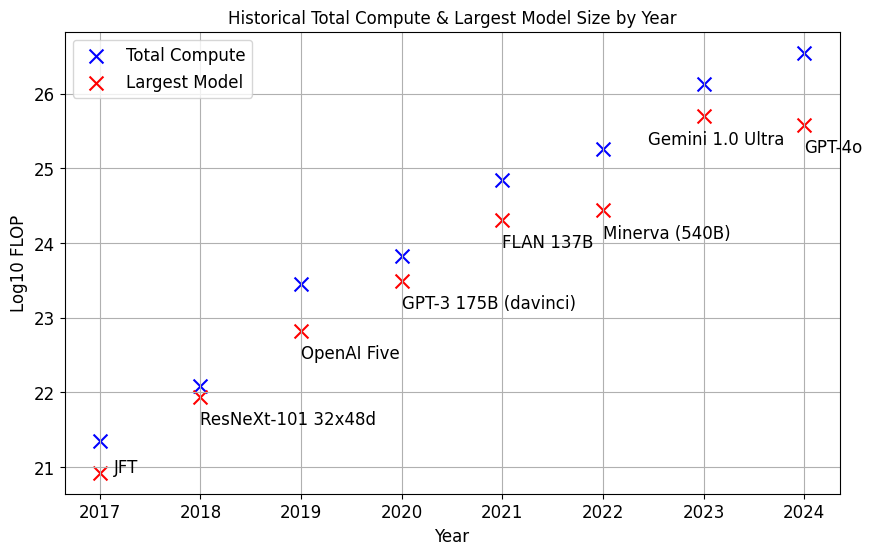
\includegraphics[width=0.8\textwidth]{media/image9.png}
\caption*{\textbf{Figure 4}: Scatter plot of the model's projected samples when all parameters are set to their median values (LMS=27.05, allocation gradient=1.0, growth rate =4.1x).}
\label{fig:model-projections}
\end{figure}

The Verification section aims to validate the model projections by retrodicting our model and comparing the results to the historically observed data. Here we find that the 90\% prediction intervals capture all historically observed data points. Taken together, this provides considerable evidence that the 90\% prediction intervals presented below are likely to capture the number of models released in the coming years above each respective threshold.

\subsection{Absolute compute thresholds}

First, we can compare our model's projections to what we know about the number of AI models exceeding 10$^{25}$ FLOP\footnote{Although we didn't use 2024 data to fit the model because it appears \hyperref[appendix-a-historical-distribution-of-notable-models-and-fit-data-choice]{incomplete}, we include this comparison as it seems that the 2024 data is incomplete towards the \textit{left tail} of the distribution. 10$^{25}$ FLOP models in 2024 are firmly on the right tail of the model distribution, making them more likely to be accounted for in the database.}. Recall that we set the largest model share parameter for 2024 to 0.1 to enforce the condition that the largest model released that year was the size of GPT-4o at 3.8x10$^{25}$ FLOP. We show a results table \textit{without this constraint} in \underline{\hyperref[appendix-e-2024-predictions-under-uniform-sampling-of-lms]{Appendix E}}. With this constraint, our model predicts a median of 16 10$^{25}$ FLOP models in 2024, which falls in the centre of the 12 counted in the latest version of the Notable Models database and the 20 estimated in \underline{\href{https://epoch.ai/data-insights/models-over-1e25-flop}{this}} article.

Assuming these prediction intervals will hold over the coming years, what are the implications for training compute thresholds? By the end of 2028 (EOY 2028) our median and 95th percentile projections for the number of models exceeding the 10$^{25}$ FLOP threshold in the EU AI Act are 127 and 287 respectively. Our median and 95th percentile projection for the number of models exceeding the 10$^{26}$ threshold in the Diffusion Framework are 63 and 134.

\begin{table}[h]
\centering
\caption*{\textbf{Table 3}: \textbf{Results for absolute thresholds.} Table 3 presents the 90\% prediction intervals for the absolute compute thresholds. The results in the table are cumulative, showing the projections for the number of models above threshold X that had been released by the end of a given year, rather than the number of models that were released in that year. For example, our 95th percentile projection for the number of models exceeding 10$^{25}$ FLOP by the end of 2025 is 57, with 19 of these released in 2024.}
\label{tab:absolute-thresholds}
\begin{tabular}{|l|c|c|c|c|c|}
\hline
\textbf{Threshold (FLOP)} & \textbf{2024} & \textbf{2025} & \textbf{2026} & \textbf{2027} & \textbf{2028} \\
\hline
\textbf{$>$ 10$^{25}$} & [13, 16, 19] & [24, 33, 57] & [39, 58, 117] & [60, 88, 192] & [81, 127, 287] \\
\hline
\textbf{$>$ 10$^{26}$} & [0, 0, 0] & [2, 6, 10] & [10, 19, 36] & [22, 37, 74] & [37, 63, 134] \\
\hline
\textbf{$>$ 10$^{27}$} & [0, 0, 0] & [0, 0, 1] & [0, 2, 5] & [1, 9, 17] & [8, 22, 47] \\
\hline
\textbf{$>$ 10$^{28}$} & [0, 0, 0] & [0, 0, 0] & [0, 0, 0] & [0, 0, 1] & [0, 3, 9] \\
\hline
\textbf{$>$ 10$^{29}$} & [0, 0, 0] & [0, 0, 0] & [0, 0, 0] & [0, 0, 0] & [0, 0, 0] \\
\hline
\end{tabular}
\end{table}

It is also worth noting the growth rate of the number of models exceeding the AI Act's threshold each year. Considering the 95th percentile projections, we see that from 2024-2025 the number of models captured by the 10$^{25}$ threshold increases by 38, and then 60, 75 and 90 in subsequent years. This highlights a superlinear growth trend; not only does the number of models captured by the Act's compute threshold increase, but it increases at a growing rate. This superlinear growth trend holds across \textit{all} projections (5th, 50th and 95th percentile forecasts) and across all absolute compute thresholds.

\subsection{Frontier-connected thresholds}

We now consider the results of our projections for the frontier-connected thresholds defined in \underline{\hyperref[frontier-connected-thresholds]{Section 2.4}}. These results are shown in \underline{\hyperref[table-4-frontier-connected-thresholds.-results-for-frontier-connected-thresholds-5th-50th-95th-percentile-projections.-2024-predictions-differ-from-2025-2028-as-we-fix-the-largest-model-in-2024-to-the-size-of-gpt-4o.-results-are-for-model-release-projections-within-the-specified-year-only.]{Table 4}}. The key takeaway is that across all projections (5th, 50th and 95th percentile) and all thresholds (within 0.5, 1.0 and 1.5 OOMs of the largest model), the number of models captured by the threshold stays roughly constant \textit{each year}\footnote{The exception in the table above is for 2024 where we set the largest model produced to be the size of GPT-4o. For the predictions \textbf{without} this constraint, see \hyperref[appendix-e-2024-predictions-under-uniform-sampling-of-lms]{Appendix E}; in this case, the 2024 frontier-connected counts follow a similar trend to 2025-2028.}. For example, our median projection for the number of models that are within 1 OOM of the largest model at a given date is stable at 9-11 models across each year from 2025-2028, and the other thresholds of 0.5 OOMs and 1.5 OOMs see a similar trend. This constancy across time in the number of models captured by the threshold may be a desirable property for regulatory bodies responsible for enforcement; however the extent to which the frontier-connected thresholds are preferable over absolute training compute thresholds will also depend on whether the risks posed by a model are due to its absolute size or it's size relative to the frontier.

\begin{table}[h]
\centering
\caption*{\textbf{Table 4: Frontier-connected thresholds.} Results for frontier-connected thresholds (5th, 50th, 95th percentile projections). 2024 predictions differ from 2025-2028 as we fix the largest model in 2024 to the size of GPT-4o. Results are for model release projections within the specified year only.}
\label{table-4-frontier-connected-thresholds.-results-for-frontier-connected-thresholds-5th-50th-95th-percentile-projections.-2024-predictions-differ-from-2025-2028-as-we-fix-the-largest-model-in-2024-to-the-size-of-gpt-4o.-results-are-for-model-release-projections-within-the-specified-year-only.}
\begin{tabular}{|l|c|c|c|c|c|}
\hline
Distance from frontier model & \textbf{2024} & \textbf{2025} & \textbf{2026} & \textbf{2027} & \textbf{2028} \\
\hline
\textbf{Within 0.5 OOM} & [8, 11, 14] & [1, 5, 18] & [2, 5, 17] & [1, 4, 13] & [2, 5, 16] \\
\hline
\textbf{Within 1 OOM} & [19, 22, 25] & [5, 10, 34] & [5, 10, 35] & [5, 9, 28] & [5, 11, 34] \\
\hline
\textbf{Within 1.5 OOM} & [30, 34, 38] & [8, 14, 54] & [8, 17, 52] & [8, 15, 44] & [8, 16, 50] \\
\hline
\end{tabular}
\end{table}

\section{Verification}

In this section we present results obtained by retrodicting our model for absolute compute thresholds 10$^{23}$, 10$^{24}$ and 10$^{25}$ FLOP, for which there exists data from the years 2020-2023. We also compare our models predictions with the number of AI models satisfying the frontier-connected thresholds. The model's 90\% prediction intervals capture all of these historically observed data points, which provides considerable evidence that the predicted intervals will capture the actual number of models exceeding the thresholds.

\subsection{Absolute compute thresholds}

\begin{table}[h]
\centering
\caption*{\textbf{Table 5}: Absolute compute thresholds retrodiction. Each cell is formatted as O (5, 50, 95) where: O - historically observed data, 5 - 5th percentile projection, 50 - 50th percentile projection, 95 - 95th percentile projection.}
\label{tab:absolute-retrodiction}
\begin{tabular}{|l|c|c|c|c|}
\hline
\textbf{Threshold (FLOP)} & \textbf{2020} & \textbf{2021} & \textbf{2022} & \textbf{2023} \\
\hline
\textbf{$>$ 10$^{23}$} & 2 (0,1,4) & 9 (8,14,27) & 29 (18,30,63) & 54 (34,54,126) \\
\hline
\textbf{$>$ 10$^{24}$} & 0 (0,0,0) & 3 (0,2,3) & 8 (2,7,10) & 19 (12,21,43) \\
\hline
\textbf{$>$ 10$^{25}$} & 0 (0,0,0) & 0 (0,0,0) & 0 (0,0,0) & 4 (0,4,5) \\
\hline
\end{tabular}
\end{table}

For the absolute compute thresholds 10$^{23}$, 10$^{24}$ and 10$^{25}$ FLOP, our 90\% confidence interval captures the historically observed values for the years 2020-2023. Note however, that for a number of cells the historically observed value is closer to the model's 5th or 95th projection than it is to the median projection, highlighting the importance of interpreting the full prediction interval.

\subsection{Frontier-connected threshold}

\begin{table}[h]
\centering
\caption*{\textbf{Table 6}: \textbf{Frontier-connected thresholds retrodiction.} Each cell is formatted as O (5, 50, 95) where: O - historically observed data, 5 - 5th percentile projection, 50 - 50th percentile projection, 95 - 95th percentile projection.}
\label{tab:frontier-retrodiction}
\begin{tabular}{|l|c|c|c|c|}
\hline
\textbf{Distance from frontier model} & \textbf{2020} & \textbf{2021} & \textbf{2022} & \textbf{2023} \\
\hline
\textbf{Within 0.5 OOM} & 3 (1,5,13) & 4 (1,5,17) & 5 (1,4,15) & 5 (1,5,17) \\
\hline
\textbf{Within 1.0 OOM} & 7 (4,10,29) & 19 (5,11,33) & 16 (4,10,30) & 11 (5,9,32) \\
\hline
\textbf{Within 1.5 OOM} & 11 (8,16,47) & 27 (8,17,49) & 22 (7,15,46) & 17 (8,14,47) \\
\hline
\end{tabular}
\end{table}

For the 0.5, 1.0 and 1.5 OOM frontier-connected thresholds, our 90\% confidence interval captures all of the historically observed values. Again, in some cases (e.g: 2021), the observed value is closer to the 5th or 95th percentile projection than it is to the median projection.

\section{Limitations}

In this section the limitations of our analysis are discussed. This includes the selection effect on the machine learning models tracked by the Notable Models database, as well as limitations resulting from uncertainty in key parameters that influence the model's predictions (such as the largest model share parameter) and compute growth rates.

\subsection{Notable models selection effect}
\label{notable-models-selection-effect}

The notable models database is a strict subset of all machine learning models. Therefore using this dataset to model future trends will, in general, lead to point estimates of the number of models that exceed the absolute compute thresholds being a lower bound on the true number\textit{.} However, the nearer a model is to the frontier, the closer this lower bound estimate will be to the actual number of models that exceed the threshold. To illustrate, consider the cases of setting a 10$^{22}$ FLOP compute threshold and 10$^{25}$ FLOP threshold in the year 2023. In 2023, the largest model released was Gemini Ultra at 5x10$^{25}$ FLOP. Most models with training compute on the order of 10$^{25}$ are likely to have satisfied at least one of the notability criteria\footnote{As a reminder, the notability criteria are:
\begin{itemize}
\item highly cited (over 1000 citations);
\item large training cost (over \$1,000,000, measured in 2023 USD);
\item significant use (over one million monthly active users);
\item state of the art performance (typically on a recognised ML benchmark);
\item indisputable historical significance.
\end{itemize}} given their proximity to the frontier AI model of the day. However, models of size $\sim$10$^{22}$ FLOP in 2023 are far less likely to have met the notability criteria and thus more likely to be excluded from the dataset, making point estimates of the trends of 10$^{22}$ FLOP models less reliable.

One way in which this effect can be accounted for within our model is by setting the allocation gradient (k) to less than one. Qualitatively this means that smaller models get more compute relative to the median scenario in our baseline case (where the median value of k is 1.0). For example, in the case where k = 1.0, models that are within 1 OOM of the largest model trained in a given year are allocated 90\% of the compute share, with models within 1 OOM and 2 OOM of the largest model getting a factor of 10 less - 9\%. On the other hand, when k = 0.5, models within 1 OOM of the frontier get only 68\% of compute, and those in the category below it get 10$^{0.5}$ $\sim$ 3.2x less (other allocations are shown in \underline{\hyperref[table-i.1---compute-allocations-for-various-k-1.-each-column-gives-the-allocation-for-a-particular-model-size-relative-to-the-largest-model-trained-in-a-given-year.-e.g-the-rightmost-column-shows-compute-allocations-for-models-within-1-oom-of-the-largest-model-size.]{Table I.1 in Appendix I}}). The results of our baseline model shown in \underline{\hyperref[results]{Section 3}} choose k based on \underline{\hyperref[appendix-d-historical-values-of-allocation-gradients]{historical values}} found from the Notable Models database as it is unclear how to modify this parameter to account for the notable models selection effect. However in \underline{\hyperref[appendix-i-results-for-varying-allocation-gradients]{Appendix I}}, results are presented in which k is sampled uniformly from the range [0.5, 1.0] to illustrate the outcome on compute thresholds when a correction for the notable models selection effect is applied.

Even within our baseline predictions (where k is sampled uniformly from [0.9,1.1]), it should be emphasised that our 90\% prediction intervals are designed to capture uncertainty in the model parameters (such as largest model share, allocation gradient, and compute stock growth rate), not the uncertainty that arises from the Notable Models selection effect. However anchoring on the full prediction intervals will insure decisions against this selection effect to some extent. In other words, whilst our median projections are biased towards underestimating the actual number of models captured by the compute thresholds, this is less likely to be the case for our 95th percentile projections.

\subsection{Uncertainty in key model parameters}

Key parameters that influence the model's predictions are the largest model share parameter (LMS), the compute stock growth rate, the allocation gradient, and the allocation of the compute stock between training and inference. Our choices for most of these parameters are informed by their historical values, for which we have limited data (2017-2023). This introduces uncertainty into our model, which we account for with 90\% confidence intervals. However the limited historical data often only provides six (6) data points to calibrate these intervals with.

For example, the LMS in previous years has varied significantly over the range 0.1 (2024) to 0.46 (2020). In making projections for the years 2025-2028 we therefore sample the LMS uniformly from a wider range of [0.05,0.5]. Given that low values of the LMS can lead to substantially different projections to larger values (\underline{\hyperref[f.2-influence-of-lms-on-projections]{Appendix F.2}} discusses this in further detail), future work could look to further calibrate this parameter as more data becomes available. The case for the compute stock growth rate is similar - the two sources of evidence that are used in this study (historical compute growth rates and Dean et al.'s\footnote{\href{https://ai-2027.com/supplements/compute-forecast}{https://ai-2027.com/supplements/compute-forecast}} forecast of future compute stock growth) show a noticeable discrepancy which we resolve by subjectively weighting the estimated growth rates. Valuable future work could look to conduct further analysis into the growth of compute that is available for AI training and inference.

\section{Implications for Compute-Threshold-Based Governance Frameworks}

Training compute is increasingly being used as a proxy for determining which AI models should be subject to requirements imposed by AI governance frameworks. As Heim and Koessler (2024) argue, compute thresholds serve as an effective initial filter to identify potentially risky general-purpose AI models that warrant regulatory oversight and further scrutiny.\footnote{\href{https://arxiv.org/abs/2405.10799}{Heim and Koessler, 2024}} This approach is valuable because training compute correlates with model capabilities and potential risks while being easily quantifiable compared to other inputs to AI development.\footnote{\href{https://arxiv.org/abs/2402.08797}{Sastry, et al. 2024}}

However, our analysis demonstrates a critical challenge: any static compute threshold will capture an increasing number of models over time. By the end of 2028, our median projections indicate that 127 models will exceed the 10$^{25}$ FLOP threshold established in the EU AI Act, and 63 models will surpass the 10$^{26}$ FLOP threshold set in the US AI Diffusion Framework. Especially relevant is the superlinear growth pattern we observe. Not only does the number of models captured by these thresholds increase yearly, but the rate of increase accelerates..

This pace of increase could strain governmental capacity to enforce and monitor requirements while potentially imposing excessive regulatory burdens on a growing number of AI developers. In response, governments have two main options. First, they can make regulatory burdens more proportionate for less risky models while increasing their regulatory capacity to handle the growing number of models in scope. Second, they can reduce the scope of requirements by excluding certain models from the regime. Both the EU AI Office in the EU and the Bureau of Industry and Security in the US have the authority to make such adjustments to the scope of their respective regulatory frameworks.

\section{Conclusion}

In this paper we estimate the number of AI models that will exceed training compute thresholds such as those proposed in the EU AI Act\footnote{\href{https://artificialintelligenceact.eu/}{EU AI Act}} and the Artificial Intelligence Diffusion Framework\footnote{\href{https://www.federalregister.gov/documents/2025/01/15/2025-00636/framework-for-artificial-intelligence-diffusion}{Federal Register :: Framework for Artificial Intelligence Diffusion}}. Our method centres around estimating the total stock of compute that will be available for AI workloads (training and inference), and then allocating the training compute stock to models of different size following trends seen from 2017-2023. We find that 80-290 models will exist by the end of 2028 that exceed a 10$^{25}$ FLOP compute threshold with a 90\% confidence interval, and 40-130 models will exist above the 10$^{26}$ FLOP threshold. For all compute thresholds defined with respect to an absolute value, the number of models exceeding the threshold increases at an accelerating (superlinear) rate.

We also analyse trends for compute thresholds that are connected to the largest frontier model at the time of their release and find for thresholds that capture models within 0.5, 1.0 and 1.5 orders of magnitude of the largest model, the median number of models captured remains roughly stable each year (at 5, 10 and $\sim$15-16 respectively) - however we have wide 90\% confidence intervals around these. We validate our predictions by predicting threshold counts for the years 2020-2023, with our 90\% confidence intervals capturing all historically observed values.

However our analysis is limited by the selection effects applied by the Notable Models database which bias our median projections towards being a lower bound on the actual number of models that will exceed the absolute compute thresholds. Additionally uncertainty around model parameters such as the largest model share (LMS), allocation gradient and compute growth rate mean that the full 90\% prediction interval should be accounted for when basing policy decisions on these results. These findings emphasize the need for policymakers and regulatory bodies to consider the rapid growth in frontier AI model counts when designing and implementing compute-based governance frameworks, ensuring they have sufficient capacity to monitor and regulate an expanding number of models while maintaining flexibility to adjust thresholds as the AI landscape evolves.

\appendix

\section{Appendix A | Historical distribution of notable models and fit data choice}
\label{appendix-a-historical-distribution-of-notable-models-and-fit-data-choice}

\begin{figure}[h]
\centering
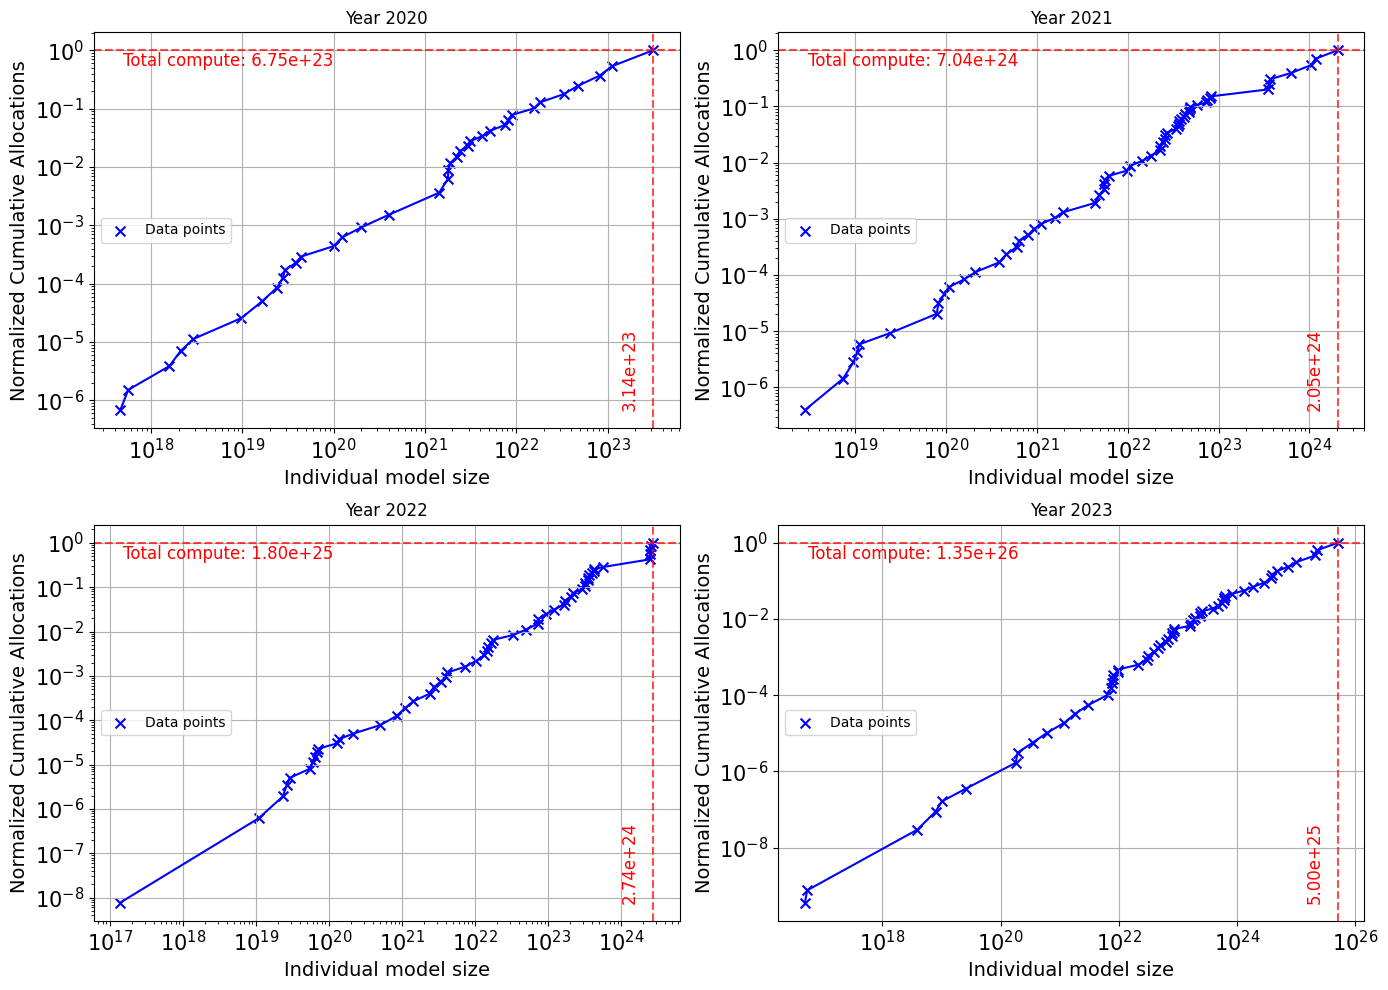
\includegraphics[width=0.8\textwidth]{media/image11.png}
\caption*{\textbf{Figure A.1}: Historical distribution of models over training compute - scatter.}
\end{figure}

The dataset we use for this analysis contains records of models and their estimated training compute dating back to the 1950s. We filter out all models that were released before 2017 as this corresponds to the era before the release of the Transformer architecture at the core of most frontier models today. Additionally, we do not use 2024 data to fit our model. Observing the model distribution in the scatter plot above, 2024 data appears incomplete relative to the previous years, especially towards the lower end of the distribution (i.e: there is a notable absence of models on the lower end of compute usage). The deviation of 2024 data from previous years can also be seen in the kernel density estimates below.

\begin{figure}[h]
\centering
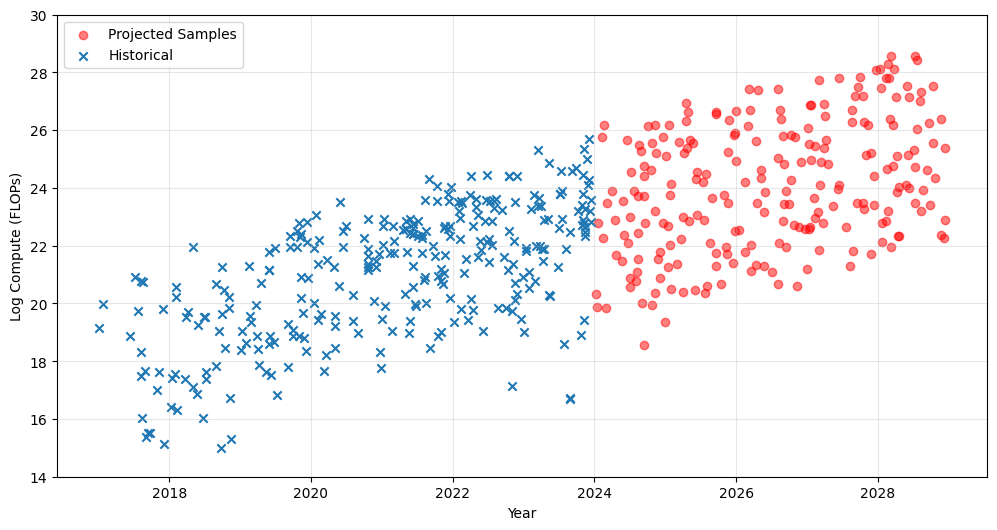
\includegraphics[width=0.6\textwidth]{media/image8.png}
\caption*{\textbf{Figure A.2}: Historical distribution of models over training compute - KDEs}
\end{figure}

\section{Appendix B | Compute allocations for 2017-2019}
\label{appendix-b-compute-allocations-for-2017-2019}

\begin{figure}[h]
\centering
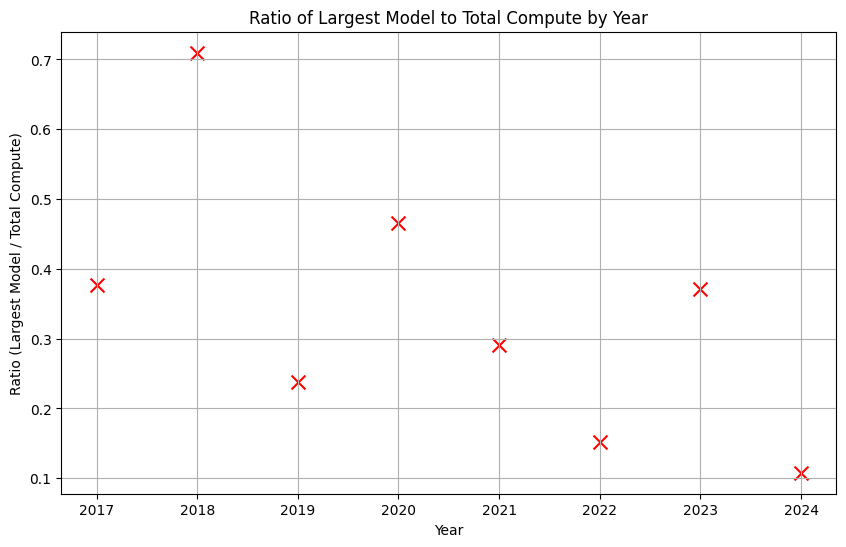
\includegraphics[width=0.8\textwidth]{media/image6.png}
\caption*{\textbf{Figure B.1}: Allocation plots for the years 2017-2019, x-axis normalised by the largest model trained that year. A similar linear trend to the 2020-2023 data is observed.}
\end{figure}

\section{Appendix C | Constraints and interpretation of the linear fits}
\label{appendix-c-constraints-and-interpretation-of-the-linear-fits}

This Appendix discusses the constraints on the linear fit to the compute allocation trends, and the interpretation of the allocation gradient parameter.

Observing historical data we see that the relationship between normalised model size (normalised by the largest model trained that year) - $\tilde{m}$ and the fraction of compute spent on models of size $\tilde{m}$ or less - denoted by $A(\tilde{m})$ - is linear in log-space. Mathematically:

$log(A(\tilde{m})) = k * log(\tilde{m}) + b $

Let that largest model trained in a given year be $m_{max}$, then $\tilde{m}_{max}$ = 1. Models of size $m_{max}$ or smaller (i.e: all models) take up all compute spending that year, therefore $A(\tilde{m}_{max} = 1) = 1$. Enforcing this constraint on 1 means that $b = 0$ - and so equation 1 reduces to $A(\tilde{m}) = \tilde{m}^k$.

The parameter $k$ determines how compute is allocated across models of different scales. To see this, let us first denote $a(m_1, m_2)$ as the amount of compute that is allocated to models in the range $[m_1, m_2)$. Consider also three sizes of models - $m^*$, $10m^*$, and $100m^*$. The compute allocated to models in the range $[m^*, 10m^*]$ is $a(m^*, 10m^*) = A(10m^*) - A(m^*) = (10^k - 1)m^{*k}$ using equation 1. The compute allocated to models in the range $[10m^*, 100m^*)$ is $a(10m^*, 100m^*) = A(100m^*) - A(10m^*) = 10^k(10^k - 1)m^{*k}$ after some simplification. Therefore the relationship between $a(m, 10m^*)$ and $a(10m^*, 100m^*)$ is simply:

$a(10m^*, 100m^*) = 10^k a(m^*, 10m^*)$

In other words, scaling up model size by a factor of 10 leads to a factor of $10^k$ increase in compute allocated to models of this size. $k = 1$ means that these larger models get 10 times as much compute as their smaller counterparts, $k > 1$ means that they get a factor greater than 10, and $k < 1$ leads to a factor less than 10.

\section{Appendix D | Historical values of allocation gradients}
\label{appendix-d-historical-values-of-allocation-gradients}

\begin{figure}[h]
\centering

\includegraphics[width=0.8\textwidth]{media/image1.png}
\caption*{\textbf{Figure D.1}: Allocation gradient parameter over time.}
\end{figure}

Historical values of the gradient of the compute allocation fits ($k$). Informed by this, our model draws $k$ uniformly from the range [0.9,1.1].

\section{Appendix E | 2024 predictions under uniform sampling of LMS}
\label{appendix-e-2024-predictions-under-uniform-sampling-of-lms}

When predicting model counts for the years 2025-2028 we sample the largest model share parameter (LMS) from the range [0.05, 0.5]. However when predicting model counts for the year 2024 we set the LMS to 0.1. This is because we have some data to inform our projections for 2024. It appears that the largest model trained during 2024 was GPT-4o at 3.8x10$^{25}$ FLOP, corresponding to an LMS parameter of roughly 0.1\footnote{How reliable is this figure given that 2024 data is incomplete? Our assumption here is that 2024 data is incomplete towards the left tail of the model distribution, but is more reliable towards the right tail of the model distribution. Given that the largest model \textbf{and} the total compute in a given year are dependent on models on the right tail of the model distribution, we take them to be sufficiently reliable to use in our projections.}. If the LMS parameter is sampled uniformly from [0.05, 0.5] for 2024, we obtain Table E.1 and Table E.2 below, in which the median projection of the number of models above 10$^{25}$ and 10$^{26}$ FLOP is 12 and 1. In other words, our model expects there to have been models exceeding 10$^{26}$ FLOP in 2024, and in predicting this sacrifices compute that instead would have gone to the 10$^{25}$ FLOP category. Observing the historical trend of the largest model and its relation to the total training compute spent that year shows that 2024 deviates from previous years, and thus our model's expectation is warranted.

\begin{figure}[h]
\centering

\includegraphics[width=0.75\textwidth]{media/image2.png}
\caption*{\textbf{Figure E.1}: Historical data for largest model and total training compute}
\end{figure}

\begin{table}[h]
\centering
\caption*{\textbf{Table E.1}: Absolute threshold predictions when 2024 LMS parameter sampled from uniformly from (0.05,0.5)}
\begin{tabular}{|l|c|c|c|c|c|}
\hline
\textbf{Threshold (FLOP)} & \textbf{2024} & \textbf{2025} & \textbf{2026} & \textbf{2027} & \textbf{2028} \\
\hline
\textbf{$>$ 10$^{25}$} & [7, 12, 19] & [18, 29, 53] & [33, 53, 112] & [51, 83, 187] & [74, 121, 283] \\
\hline
\textbf{$>$ 10$^{26}$} & [0, 1, 2] & [4, 6, 12] & [13, 20, 37] & [23, 38, 79] & [38, 64, 135] \\
\hline
\textbf{$>$ 10$^{27}$} & [0, 0, 0] & [0, 0, 1] & [0, 2, 6] & [3, 9, 20] & [10, 23, 46] \\
\hline
\textbf{$>$ 10$^{28}$} & [0, 0, 0] & [0, 0, 0] & [0, 0, 0] & [0, 0, 1] & [0, 3, 8] \\
\hline
\textbf{$>$ 10$^{29}$} & [0, 0, 0] & [0, 0, 0] & [0, 0, 0] & [0, 0, 0] & [0, 0, 0] \\
\hline
\end{tabular}
\end{table}

\begin{table}[h]
\centering
\caption*{\textbf{Table E.2}: Frontier-connected threshold predictions when 2024 LMS parameter sampled from Unif(0.05,0.5).}
\begin{tabular}{|l|c|c|c|c|c|}
\hline
\textbf{Distance from frontier model} & \textbf{2024} & \textbf{2025} & \textbf{2026} & \textbf{2027} & \textbf{2028} \\
\hline
\textbf{Within 0.5 OOM} & [2, 4, 15] & [2, 4, 14] & [2, 5, 15] & [2, 6, 15] & [2, 5, 16] \\
\hline
\textbf{Within 1 OOM} & [5, 9, 29] & [4, 9, 31] & [5, 10, 29] & [5, 12, 31] & [5, 10, 34] \\
\hline
\textbf{Within 1.5 OOM} & [8, 15, 49] & [7, 14, 48] & [8, 15, 49] & [9, 18, 53] & [8, 16, 53] \\
\hline
\end{tabular}
\end{table}

\section{Appendix F | LMS parameter and influence of LMS on projections}

\subsection{Historical LMS}
\label{f.1-historical-lms}

\begin{figure}[h]
\centering
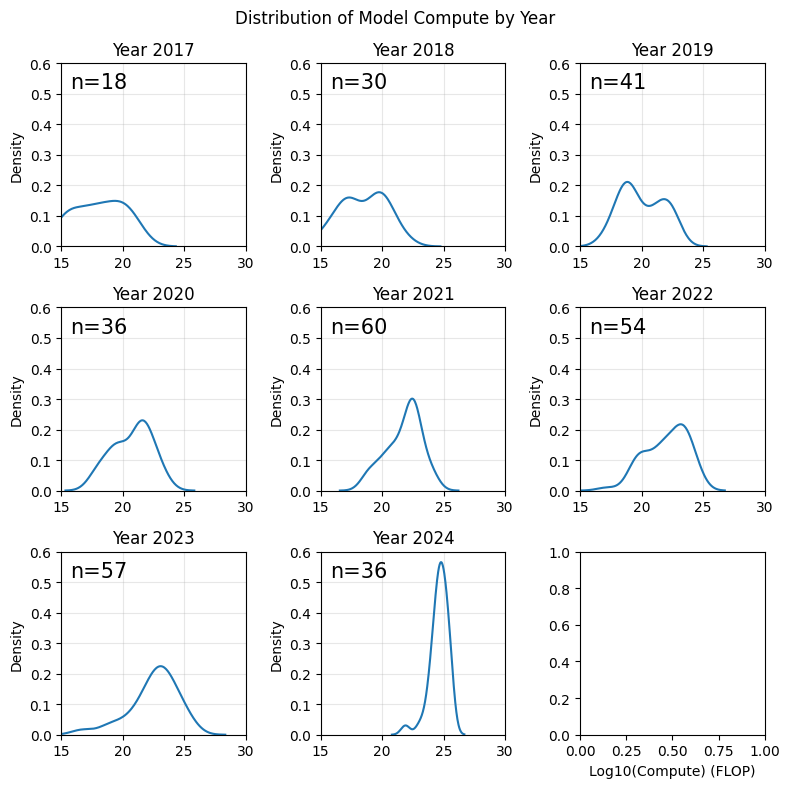
\includegraphics[width=0.75\textwidth]{media/image10.png}
\caption*{\textbf{Figure F.1:} Historical data for the largest model share parameter}
\end{figure}

\begin{figure}[h]
\centering

\includegraphics[width=0.75\textwidth]{media/image2.png}
\caption*{\textbf{Figure F.2}: Historical data for largest model and total training compute.}
\end{figure}

Historical values of the LMS parameter and the total compute and largest model each year that the LMS is derived from. AlphaGo, AlphaGo Zero and AlphaGo Master have been removed from the dataset as they represent outliers in model size. We fit the model on data from 2017-2023 and ignore the LMS for 2018 as it appears to be an outlier.

Our predictions sample the LMS uniformly from the range [0.05,0.5]. The upper bound is chosen to accommodate GPT-3 davinci accounting for $\sim$46\% of training compute in 2021. The lower bound is chosen with the 2022 value of 0.15 in mind, however we incorporate a wide range underneath this value due to the strong influence of low LMS values on the model's predictions (see Appendix F.2 below).

\subsection{Influence of LMS on projections}
\label{f.2-influence-of-lms-on-projections}

When experimenting with the model, we find that the \textbf{number} of models that exceed the compute thresholds grows large as the LMS parameter tends to 0. This appendix explores in further detail why this is the case with a toy example.

Consider the following setup. We have $10^{30}$ FLOP of compute allocated to training models in a given year. The assignment of compute amongst model sizes is shown in the table below. (note that we assume that increasing the model size by a factor of 10 grants it 10x as much compute - corresponding to k=1 for the allocation plot gradient).

\begin{table}[h]
\centering
\begin{tabular}{|l|c|c|c|c|}
\hline
Model size (in relation to largest model) & Within 3-4 OOM & Within 2-3 OOM & Within 1-2 OOM & Within 1 OOM \\
\hline
Fractional allocation & 0.009\% & 0.9\% & 9\% & 90\% \\
\hline
Allocation (FLOP) & $9\times10^{26}$ & $9\times10^{27}$ & $9\times10^{28}$ & $9\times10^{29}$ \\
\hline
\end{tabular}
\end{table}

Now let us consider two cases: one in which the LMS = 0.05, and another in which the LMS = 0.5. In scenario 1, the largest model trained that year is $0.05\times10^{30}$ = $5\times10^{28}$ FLOP, and in scenario two the largest model is $0.5\times10^{30}$ = $5\times10^{29}$ FLOP. Now consider the number of models that can be drawn from each category. To approximate this we find the average model size of each category\footnote{By taking the geometric mean of the model category bounds. We take the geometric mean instead of the arithmetic mean as the bounds are given in logspace.} - $m_{avg}$ - and find how many times $m_{avg}$ can be sampled from the compute allocations given in row three of the table above. [This is show in the tables below\textbf{.}]

In the case where the LMS=0.05, approximately 56 models of size $m_{avg}$ can be sampled for each category, compared to the 5 sampled from each category for the case of LMS=0.5. More generally, the number of average sized models that can be sampled from each category grows inversely with the \textit{size} of the average model - and the average sized model of a category grows proportionally with the LMS parameter.

\textbf{Scenario 1 - LMS=0.05}

\begin{table}[h]
\centering
\begin{tabular}{|l|c|c|c|c|c|}
\hline
Model size (in relation to largest model) & Within 3-4 OOM & Within 2-3 OOM & Within 1-2 OOM & Within 1 OOM & \\
\hline
Model size (FLOP) & 5x10$^{24}$-5x10$^{25}$ & 5x10$^{25}$-5x10$^{26}$ & 5x10$^{26}$-5x10$^{27}$ & 5x10$^{27}$-5x10$^{28}$ & \\
\hline
Average\footnote{Geometric mean} model size (FLOP) & 1.6x10$^{24}$ & 1.6x10$^{25}$ & 1.6x10$^{26}$ & 1.6x10$^{27}$ & \\
\hline
Allocation & 9x10$^{26}$ & 9x10$^{27}$ & 9x10$^{28}$ & 9x10$^{29}$ & \\
\hline
Number of samples drawn & 56 & 56 & 56 & 56 & 224 (TOTAL) \\
\hline
\end{tabular}
\end{table}

\textbf{Scenario 2 - LMS=0.5}

\begin{table}[h]
\centering
\begin{tabular}{|l|c|c|c|c|c|}
\hline
Model size (in relation to largest model) & Within 3-4 OOM & Within 2-3 OOM & Within 1-2 OOM & Within 1 OOM & \\
\hline
Model size (FLOP) & 5x10$^{25}$-5x10$^{26}$ & 5x10$^{26}$-5x10$^{27}$ & 5x10$^{27}$-5x10$^{28}$ & 5x10$^{28}$-5x10$^{29}$ & \\
\hline
Average\footnote{Geometric mean} model size & 1.6x10$^{25}$ & 1.6x10$^{26}$ & 1.6x10$^{27}$ & 1.6x10$^{28}$ & \\
\hline
Allocation & 9x10$^{26}$ & 9x10$^{27}$ & 9x10$^{28}$ & 9x10$^{29}$ & \\
\hline
Number of samples drawn & 5 & 5 & 5 & 5 & 20 (TOTAL) \\
\hline
\end{tabular}
\end{table}

\begin{figure}[h]
\centering

\includegraphics[width=0.8\textwidth]{media/image3.png}
\caption*{\textbf{Figure F.3} Left: The average-sized model for each category of model size for LMS = 0.05, 0.1 and 0.5. Right: The number of average-sized models that can be drawn from a given compute allocation for LMS = 0.05, 0.1 and 0.5.}
\end{figure}

The information in the table below is shown graphically above, alongside another configuration where the LMS=0.1. We see that the LMS determines the size of each model category - when the LMS=0.5 the average size of a model in the largest category is 1.6x10$^{29}$ FLOP whereas when the LMS = 0.1 and 0.05, the average size of a model in the largest category is 9.5x10$^{28}$ and 1.6x10$^{28}$ respectively. The number of samples that can be drawn given the compute allocations derived above is shown in the right hand side plot - for each category, roughly 50 samples can be drawn when the LMS=0.05, 30 when the LMS=0.1 and 5 when the LMS = 0.5 (the number of samples drawn from each category is constant across model sizes in the plot above because we choose an allocation gradient of k=1.)

\section{Appendix G | Results for varying growth rate weightings}
\label{appendix-g-results-for-varying-growth-rate-weightings}

Two sources of evidence inform the growth rates in the baseline scenario - the historical growth rate of training compute stocks and the compute forecast of Dean et al\footnote{\href{https://ai-2027.com/research/compute-forecast}{Compute Forecast --- AI 2027}}. The baseline scenario gives three times as much weight to the latter (ascribing weights of 0.25 and 0.75 to each respective growth rate), but these are subjective judgements. This Appendix shows predictions for other choices of growth rate weightings - namely weightings of (0.1,0.9), (0.33, 0.66) and (0.5, 0.5).

\begin{table}[h]
\centering
\caption*{\textbf{Table G.1} - Results for growth rate weighting of (0.1,0.9)}
\begin{tabular}{|l|c|c|c|c|c|}
\hline
\textbf{Threshold (FLOP)} & \textbf{2024} & \textbf{2025} & \textbf{2026} & \textbf{2027} & \textbf{2028} \\
\hline
\textbf{$>$ 10$^{25}$} & [12, 15, 18] & [22, 33, 53] & [35, 55, 105] & [51, 81, 175] & [69, 114, 254] \\
\hline
\textbf{$>$ 10$^{26}$} & [0, 0, 0] & [0, 5, 8] & [6, 16, 26] & [15, 31, 59] & [26, 52, 108] \\
\hline
\textbf{$>$ 10$^{27}$} & [0, 0, 0] & [0, 0, 0] & [0, 1, 3] & [0, 5, 11] & [4, 15, 34] \\
\hline
\textbf{$>$ 10$^{28}$} & [0, 0, 0] & [0, 0, 0] & [0, 0, 0] & [0, 0, 0] & [0, 0, 4] \\
\hline
\textbf{$>$ 10$^{29}$} & [0, 0, 0] & [0, 0, 0] & [0, 0, 0] & [0, 0, 0] & [0, 0, 0] \\
\hline
\end{tabular}
\end{table}

\begin{table}[h]
\centering
\caption*{\textbf{Table G.2} - Results for growth rate weighting of (0.33,0.66)}
\begin{tabular}{|l|c|c|c|c|c|}
\hline
\textbf{Threshold (FLOP)} & \textbf{2024} & \textbf{2025} & \textbf{2026} & \textbf{2027} & \textbf{2028} \\
\hline
\textbf{$>$ 10$^{25}$} & [14, 17, 20] & [26, 35, 65] & [41, 61, 135] & [59, 93, 215] & [85, 135, 320] \\
\hline
\textbf{$>$ 10$^{26}$} & [0, 0, 0] & [4, 7, 10] & [12, 21, 41] & [24, 41, 85] & [41, 70, 150] \\
\hline
\textbf{$>$ 10$^{27}$} & [0, 0, 0] & [0, 0, 1] & [0, 3, 7] & [5, 11, 23] & [14, 27, 55] \\
\hline
\textbf{$>$ 10$^{28}$} & [0, 0, 0] & [0, 0, 0] & [0, 0, 0] & [0, 0, 2] & [0, 5, 12] \\
\hline
\textbf{$>$ 10$^{29}$} & [0, 0, 0] & [0, 0, 0] & [0, 0, 0] & [0, 0, 0] & [0, 0, 0] \\
\hline
\end{tabular}
\end{table}

\begin{table}[h]
\centering
\caption*{\textbf{Table G.3} - Results for growth rate weighting of (0.5,0.5)}
\begin{tabular}{|l|c|c|c|c|c|}
\hline
\textbf{Threshold (FLOP)} & \textbf{2024} & \textbf{2025} & \textbf{2026} & \textbf{2027} & \textbf{2028} \\
\hline
\textbf{$>$ 10$^{25}$} & [15, 17, 21] & [28, 37, 72] & [45, 63, 139] & [66, 96, 212] & [89, 136, 341] \\
\hline
\textbf{$>$ 10$^{26}$} & [0, 0, 0] & [5, 8, 13] & [15, 23, 46] & [28, 45, 91] & [45, 72, 174] \\
\hline
\textbf{$>$ 10$^{27}$} & [0, 0, 0] & [0, 0, 1] & [0, 4, 8] & [6, 14, 26] & [17, 30, 68] \\
\hline
\textbf{$>$ 10$^{28}$} & [0, 0, 0] & [0, 0, 0] & [0, 0, 0] & [0, 0, 3] & [0, 6, 14] \\
\hline
\textbf{$>$ 10$^{29}$} & [0, 0, 0] & [0, 0, 0] & [0, 0, 0] & [0, 0, 0] & [0, 0, 1] \\
\hline
\end{tabular}
\end{table}

\section{Appendix H - Results for alternate training compute allocations}
\label{appendix-h---results-for-alternate-training-compute-allocations}

\hyperref[allocating-compute-between-training-inference-and-other-workloads]{Section 2.3} highlighted that the publicly available information on the allocation of compute between training, inference and other workloads was conflicting. Our baseline model uses a slightly adjusted version of the allocation in Dean et al\footnote{\href{https://ai-2027.com/supplements/compute-forecast}{https://ai-2027.com/supplements/compute-forecast}}. However another source for the compute allocations is the Epoch GATE model\footnote{\href{https://epoch.ai/gate}{https://epoch.ai/gate} - See inference-training split graph. Note that the GATE model forecasts the allocation of effective compute - which is the physical compute stock multiplied by algorithmic progress. However in the near future (e.g: 2025-2028), these two quantities do not substantially differ.}; the allocations for this model are shown below.

\begin{table}[h]
\centering
\caption*{\textbf{Table H.1} - GATE model compute allocations for training, 2025-2028}
\begin{tabular}{|l|c|}
\hline
Year & Approximate training compute allocations (GATE) \\
\hline
2025 & 90\% \\
\hline
2026 & 70\% \\
\hline
2027 & 70\% \\
\hline
2028 & 70\% \\
\hline
\end{tabular}
\end{table}

It's clear that these forecasts differ substantially to those in AI 2027, however it is out of scope for this article to explore why. This Appendix shows the predictions of the model for the absolute compute thresholds when training compute allocations are set as above.

\begin{table}[h]
\centering
\caption*{\textbf{Table H.2} - Predictions under GATE model allocations}
\begin{tabular}{|l|c|c|c|c|c|}
\hline
\textbf{Threshold (FLOP)} & \textbf{2024} & \textbf{2025} & \textbf{2026} & \textbf{2027} & \textbf{2028} \\
\hline
\textbf{$>$1e25} & [21, 24, 28] & [35, 45, 75] & [50, 69, 137] & [69, 98, 217] & [94, 140, 331] \\
\hline
\textbf{$>$1e26} & [0, 2, 5] & [6, 12, 23] & [15, 26, 52] & [28, 45, 102] & [45, 74, 178] \\
\hline
\textbf{$>$1e27} & [0, 0, 0] & [0, 0, 2] & [0, 4, 10] & [6, 14, 31] & [16, 32, 70] \\
\hline
\textbf{$>$1e28} & [0, 0, 0] & [0, 0, 0] & [0, 0, 0] & [0, 1, 4] & [0, 7, 20] \\
\hline
\textbf{$>$1e29} & [0, 0, 0] & [0, 0, 0] & [0, 0, 0] & [0, 0, 0] & [0, 0, 1] \\
\hline
\end{tabular}
\end{table}

\section{Appendix I | Results for varying allocation gradients}
\label{appendix-i-results-for-varying-allocation-gradients}

\begin{table}[h]
\centering
\caption*{\textbf{Table I.1} - Compute allocations for various k $<$ 1. Each column gives the allocation for a particular model size, relative to the largest model trained in a given year. E.g: The rightmost column shows compute allocations for models within 1 OOM of the largest model size.}
\begin{tabular}{|c|c|c|c|c|c|c|c|}
\hline
 & 10$^{-7}$-10$^{-6}$ & 10$^{-7}$-10$^{-^}$ & 10$^{-5}$-10$^{-4}$ & 10$^{-4}$-10$^{-3}$ & 10$^{-3}$-10$^{-2}$ & 10$^{-2}$-10$^{-1}$ & 10$^{-1}$-10$^{0}$ \\
\hline
k=0.5 & 0.068 & 0.22 & 0.68 & 2.2 & 6.8 & 22 & 68 \\
\hline
k=0.6 & 0.019 & 0.075 & 0.3 & 1.2 & 4.7 & 19 & 75 \\
\hline
k=0.7 & 0.0051 & 0.0025 & 0.13 & 0.64 & 3.2 & 16 & 80 \\
\hline
k=0.8 & 0.0013 & 0.0084 & 0.53 & 0.34 & 2.1 & 13 & 84 \\
\hline
k=0.9 & 0.00035 & 0.0028 & 0.022 & 0.17 & 1.4 & 11 & 87 \\
\hline
k=1.0 & 0.00009 & 0.0009 & 0.009 & 0.09 & 0.9 & 9 & 90 \\
\hline
\end{tabular}
\end{table}

Our baseline scenario samples the allocation gradient uniformly from the range [0.9, 1.1]. The median prediction in this scenario will therefore follow a compute allocation across model sizes as shown in the k=1 scenario in the table above. This modelling choice is made from observations of the allocation plots for the Notable models released in the \underline{\hyperref[appendix-d-historical-values-of-allocation-gradients]{years 2017-2023}}.

However section 5.2 discusses the limitations of the Notable Models database upon which these trends are based. One way to account for the Notable Models selection effect is to allocate more compute to smaller models relative to their larger counterparts. This can be seen in the table above where the k=0.5 case allocates $\sim$68\% of compute that year to the largest model category, whereas the k=1.0 case allocates 90\% of compute. More generally, increasing model size by 10x leads to a 10$^k$ times increase in compute allocated, as shown in \underline{\hyperref[appendix-c-constraints-and-interpretation-of-the-linear-fits]{Appendix C}}.

This Appendix presents model predictions for allocation gradients that allocate relatively more compute to smaller model sizes. Specifically, the table below presents the results of our model if the allocation gradient is sampled uniformly from the range [0.5, 0.1]. Noticeably more aggressive median predictions and wider confidence intervals can be observed.

\begin{table}[h]
\centering
\caption*{\textbf{Table I.2}: Predictions when allocation gradient (k) sampled uniform from range [0.5, 1.0], as an approximate correction mechanism to notable models selection effect.}
\begin{tabular}{|l|c|c|c|c|c|}
\hline
\textbf{Threshold (FLOP)} & \textbf{2024} & \textbf{2025} & \textbf{2026} & \textbf{2027} & \textbf{2028} \\
\hline
\textbf{$>$ 10$^{25}$} & [11, 15, 18] & [24, 37, 55] & [41, 73, 145] & [61, 113, 265] & [87, 187, 510] \\
\hline
\textbf{$>$ 10$^{26}$} & [0, 0, 0] & [3, 5, 8] & [11, 18, 33] & [23, 38, 76] & [39, 73, 172] \\
\hline
\textbf{$>$ 10$^{27}$} & [0, 0, 0] & [0, 0, 0] & [0, 2, 4] & [2, 8, 15] & [10, 22, 47] \\
\hline
\textbf{$>$ 10$^{28}$} & [0, 0, 0] & [0, 0, 0] & [0, 0, 0] & [0, 0, 1] & [0, 2, 7] \\
\hline
\textbf{$>$ 10$^{29}$} & [0, 0, 0] & [0, 0, 0] & [0, 0, 0] & [0, 0, 0] & [0, 0, 0] \\
\hline
\end{tabular}
\end{table}

\end{document}